\chapter{Natural Language Processing}
\label{cha:NaturalLanguageProcessing}
\section{Überblick}
In diesem Kapitel wird ein grober Überblick über den Ablauf beim \textit{NLP} gegeben und außerdem einige Beispiele gezeigt, die bereits im IT-Umfeld eingesetzt werden. 

\section{Verarbeitung und Interpretation von natürlicher Sprache}
\label{sec:applications-natural-language-processing}
Grundsätzlich ist Basis jeder \textit{NLP-Engine} die Verarbeitung und Interpretierung von geschriebener Sprache. Dabei ist zu unterscheiden, aus welcher Quelle der Input für die Verarbeitung kommt. Meist wird hier zwischen zwei Teilgebieten unterschieden:

\begin{itemize}
	\item Maschinenlesbare Texte
	\item Spracheingabe
\end{itemize}

Diese beiden Teilgebiete unterscheiden sich darin, dass bei der Spracheingabe noch eine Vorverarbeitung stattfinden muss, sodass der gesprochene Text interpretiert werden kann. Sobald der gesprochene Text in Form eines maschinenlesbaren Textes vorliegt, kann mit der Weiterverarbeitung begonnen werden. Dies bedeutet im Umkehrschluss, dass beide Teilgebiete auf der gleichen Engine basieren können, sich jedoch in ihrer Komplexität und der Möglichkeit der Eingabe unterscheiden. 

Im Folgenden wird kurz erläutert, wie der Ablauf einer Analyse im \textit{NLP} vom Input bis zum Output abläuft. 

\subsection{Eingabe von Sprache und Vorverarbeitung}
Die Eingabe von Sprache für das \textit{NLP} kann auf mehrere verschiedene Arten erfolgen. Es gibt die Möglichkeit, über ein Mikrofon Lautsprache aufzunehmen, oder verschiedene Texte als Input zu verwenden. Dabei könnten zum Beispiel Texte automatisch von Internetseiten ausgelesen, oder auch Dokumente am Rechner durchsucht werden. Eine weitere Möglichkeit für textuellen Input lässt sich in Form eines Chats finden. Hier findet eine textuelle Eingabe statt, die später von einer Engine verarbeitet werden kann. 

Prinzipiell unterscheiden sich diese beiden Eingabemöglichkeiten sehr stark in ihrer Komplexität. Bei der Eingabe über Lautsprache muss beim Einlesen nicht nur auf das Erkennen der Wörter, sondern auf eine etwaige Fehlerkorrektur durch Unterbrechungen oder Nebengeräusche geachtet werden. Durch diese Probleme gestaltet sich die Spracherkennung als sehr schwierig, wodurch die Möglichkeiten der Anwendung sehr stark eingeschränkt werden. Nicht zuletzt durch die Tatsache, dass in den letzten Jahren sehr viel auf dem Gebiet der Spracherkennung geforscht wurde, konnte im vergangen Jahr ein Erfolg auf diesem Gebiet erreicht werden. Einem Forschungsteam der Firma Microsoft ist es gelungen, eine \textit{Word error rate} von 5,9\% zu erreichen, was ungefähr der Fehlerrate entspricht, die bei der normalen zwischenmenschlichen Kommunikation auftritt \cite{Xiong2016}. 

\subsection{Vorverarbeitung und Information Extraction}
Sobald Text in maschinenlesbarer Form vorliegt (z.B. ASCII-Code) kann auf den syntaktischen bzw. den semantischen Inhalt geprüft werden. Dazu gibt es verschiedene Möglichkeiten für die sogenannte \textit{Information Extraction}. Ein Beispiel dafür ist die sogenannte \textit{Named Entity Recognition (NER)}. \textit{NER} ermöglicht das Verarbeiten der Texte und liefert Informationen über den Inhalt der Texte. Ergebnis der \textit{NER} sind die sogenannten \textit{Entities}. Es handelt sich dabei um Personen oder Objekte, welche in dem zu analysierenden Text enthalten sind. Es werden außerdem Attribute der Entities, wie zum Beispiel das Alter, extrahiert. Für eine genauere Analyse können auch Beziehungen zwischen Entities oder Ereignisse in welche Entities einbezogen sind ausgelesen werden. Diese Informationen können für die weitere Verarbeitung und Interpretation verwendet werden und je nach Genauigkeit der ausgelesenen Daten kann die Qualität der Aussage die über den Inhalt getroffen werden kann variieren. In der untenstehenden Grafik ist der Ablauf eines \textit{NER} Zyklus dargestellt.

\begin{figure}[ht]
	\centering
		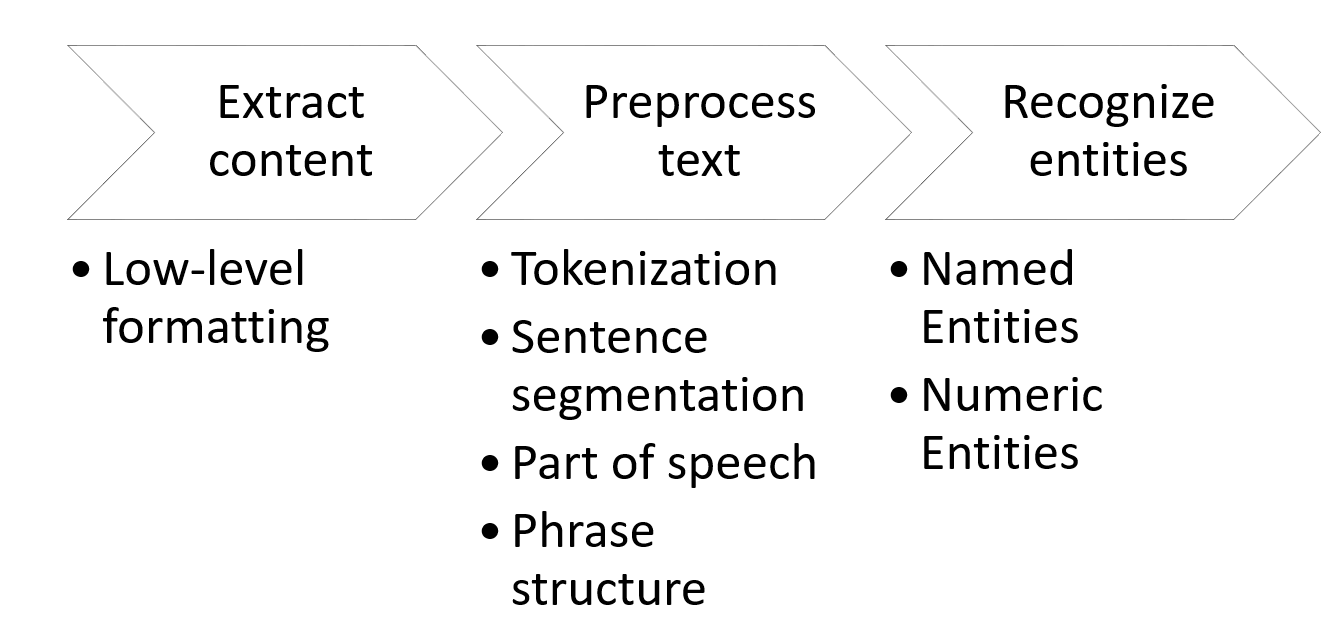
\includegraphics[width=0.80\textwidth]{images/ner-pipeline.PNG}
	\caption{Named Entity Recognition Prozess}
	\label{fig:ner-pipeline}
\end{figure}

Der in Abbildung \ref{fig:ner-pipeline} dargestellte NER Prozesses zeigt sehr gut, wie der normale Ablauf bei der Texterkennung erfolgt. Zuerst wird der Text verarbeitet, dazu werden unnötige Zeichen entfernt; Bilder, Werbung und andere Objekte mit keiner semantischen Bedeutung werden ebenfalls entfernt. Danach wird der Text vorverarbeitet. Es werden dazu einzelne Tokens gebildet, wobei jeder Token ein Wort repräsentiert. Diese Tokens werden wiederum zu Sätzen zusammengefasst, sodass die semantische Bedeutung nicht verloren geht. Sobald Sätze gebildet wurden, erfolgt das sogenannte \textit{Part-of-speech-tagging}. Beim \textit{Part-of-speech-tagging} wird festgestellt, welche verschiedenen Wortarten die Tokens darstellen und die Tokens bekommen ein Label mit der jeweiligen Wortart. Dies dient vor allem der besseren semantischen Interpretation. Im letzten Schritt der Vorverarbeitung wird die grammatikalische Struktur des Satzes in Form eines Baumes abgebildet. Sobald alle Schritte abgeschlossen sind werden die einzelnen sogenannten Entities ausgelesen. Man unterscheidet hierbei zwischen \textit{Named Entities}, es handelt sich dabei um Objekte wie z.B. Personen, oder um \textit{Numeric Entities}, welche z.B. Jahreszahlen repräsentieren. Mit diesen Informationen kann schließlich eine weitere Interpretation auf den semantischen Inhalt dieses Textes erfolgen.

\subsection{Interpretation}
Der letzte Schritt bei der Verarbeitung von natürlicher Sprache ist die Interpretation des Inhaltes. Dabei werden die extrahierten Informationen mittels Algorithmus so vernetzt, dass Aussagen über den Inhalt getroffen werden können. Dieser Teilaspekt des \textit{NLP} ist sehr vielseitig und abhängig von der Komplexität der Anforderung. Es können hier von einfachen logischen Überprüfungen bis zu der Anwendung von künstlicher Intelligenz ein breites Spektrum an Algorithmen verwendet werden. 

\subsection{Ausgabe und Ergebnis}
Am Ende sollte je nach Anforderung bzw. Anwendung ein Text ausgegeben, ein Ereignis getriggert, oder weitere Schritte eingeleitet werden. In den nächsten Abschnitten werden einige Möglichkeiten der Anwendung von \textit{NLP} erläutert, die bereits in IT-Prozessen Anwendung finden oder eventuell verwendet werden könnten. 

\section{Anwendungen von Natural Language Processing}
Nachdem im letzten Abschnitt grob skizziert wurde, wie die Verarbeitung und Interpretation von natürlicher Sprache stattfindet, wird im Folgenden auf verschiedene Beispiele für Anwendungen von \textit{NLP} im IT-Bereich eingegangen.

\subsection{Chatbots}
Ein Bereich in dem die automatisierte Texterkennung verstärkt Anwendung findet, sind sogenannte Bots. Die Bots könnten dabei z.B. den First-Level Support ersetzen und grundlegende Fragen klären, wie die Art des Problems, etwaige Kontaktdaten oder auch die Dringlichkeit des Problems. Es findet dabei eine bidirektionale Kommunikation zwischen dem Kunden und einem Bot statt. Der Kunde schreibt eine Nachricht, der Bot versucht diese zu interpretieren und weitere Fragen zu erschließen. Moderne Bots bieten hier zusätzlich die Möglichkeit, dass der aktuelle Kontext persistent ist, was zur Folge hat, dass die Konversation durch die bereits gestellten Fragen und erhaltenen Antworten angepasst wird. 

\begin{figure}[ht]
	\centering
		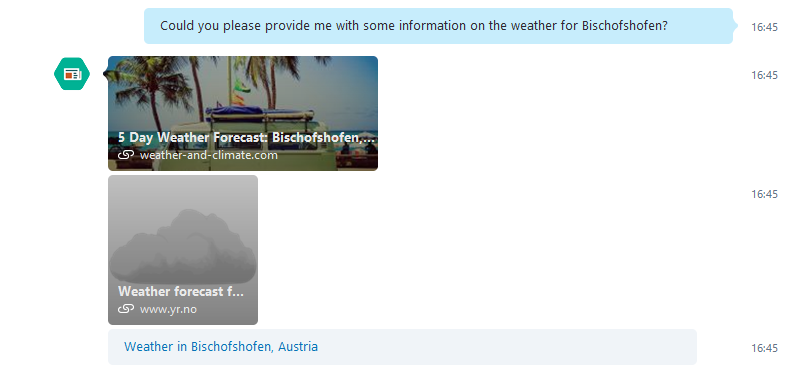
\includegraphics[width=0.80\textwidth]{images/chatbot.PNG}
	\caption{Bingnews Skype bot}
	\label{fig:chatbot}
\end{figure}

In Abbildung \ref{fig:chatbot} ist beispielhaft dargestellt, wie mit Hilfe der Texterkennung analysiert wird, welche Beiträge der Anwender gerne sehen möchte. Es werden danach die Artikel übermittelt, welche am besten mit den gesuchten Begriffen übereinstimmen. 

\subsection{Spam-Filter}
Eine äußerst bekannte und sehr weit verbreitete Anwendung von \textit{NLP} sind Spam-Filter. In der Vergangenheit wurde bei Spam-Filtern lediglich ein Whitelisting bzw. Blacklisting für verschiedene Absender oder Wörter betrieben. Sobald eine Email von einem Absender kommt, der sich auf einer Blacklist befindet, wird diese als Spam markiert. Selbiges gilt für Emails mit gewissem Inhalt, der darauf schließen lässt, dass es sich bei der Email höchstwahrscheinlich um Spam handelt. In den letzten Jahren konnte bei der Verarbeitung von Emails durch die Anwendung von \textit{NLP} eine Verbesserung bei der Erkennung und Verwaltung von Spam erreicht werden wie z.B. in \cite{Rohit2014} erläutert. 

\subsection{Sprachassistenten}
Bereits seit einigen Jahren erfreuen sich die zahlreichen Sprachassistenten immer größter Beliebtheit. Siri (Apple), Alexa (Amazon) und Cortana (Microsoft) sind dabei nur einige wenige Produkte, welche durch einen immer weiterwachsenden Funktionsumfang und eine immer tiefere Integration in vorhandene Systeme verstärkt auch im Unternehmensumfeld Anwendung finden. Dabei wird vor allem Cortana im Windows Umfeld sehr stark von Microsoft beworben und zahlreiche neue Möglichkeiten geschaffen, wie der Arbeitsalltag erleichtert werden sollte. Das Spektrum reicht dabei von der Suche nach Dokumenten, bis zum Planen von Terminen inkl. einer Rückmeldung, falls der gewünschte Zeitpunkt nicht möglich ist. Dabei ist eine sehr starke Verknüpfung mit den unterschiedlichen Systemen wie z.B. Exchange oder Office 365 erforderlich. 

Im Folgenden wird ein Beispiel skizziert, welches mit Hilfe des von Microsoft entwickelten Sprachassistenten Cortana getestet wurde. Prinzipiell ist dieses Szenario auch mit anderen Sprachassistenten möglich.

Der Anwender möchte beispielsweise einen Termin für den 30. Oktober 2017 um 10:00 Uhr planen. Cortana reagiert dabei auf die Spracheingabe und nach einer erfolgreichen Verarbeitung der Eingabe, wird in Exchange überprüft, ob der Termin belegt ist. Für diesen Tag ist bereits ein Termin eingeplant und Cortana startet eine bi-direktionale Kommunikation, indem dem Anwender mitgeteilt wird, dass der Termin bereits belegt ist und einige verschiedene Optionen aufgezeigt werden. Der Anwender entscheidet sich dafür, dass der Termin der bereits vorhanden ist verschoben wird. In einer Rückmeldung informiert Cortana den Anwender, dass der Termin verschoben und der neue Termin eingetragen wurde. Cortana erkundigt sich, ob alle Teilnehmer des verschobenen Termins informiert werden sollten. Der Anwender antwortet mit Ja und Cortana leitet im Hintergrund die nötigen Schritte ein.

Dieser Fall zeigt nur eines der Beispiele, in denen ein Sprachassistent auch im Unternehmensumfeld Anwendung finden kann. 



